%\section{Baseline Methods}
%\label{sec:method}
%In this section, we first formulate the tasks and propose two kinds of baseline methods in the two following sections, feature-based methods and LSTM-based methods.
%
\section{Sentence-level \lnear~Relation Classification}
\label{sec:classify} 
%\textbf{Problem Statement} 
Given a sentence $s$ mentioning a pair of physical objects 
\textless$e_i,e_j$\textgreater, we call \textless$s,e_i,e_j$\textgreater
~an {\em instance}. 
In this section, we aim to 
determine whether $e_i$ and $e_j$ are located near each other in a physical scene described in the sentence $s$.
For example, suppose $e_i$ is ``dog", $e_j$ is ``cat'', and $s$ = ``\textit{The King puts his dog and cat on the table.}''.
As it is true that the two objects are located near in this sentence, a successful classification model is expected to label this instance as \textit{True}.
%and
While if $s_2$ = ``\textit{My dog is older than her cat.}'', then the answer to the instance \textless$s_2,e_i,e_j$\textgreater ~is \textit{False}, for $s_2$ is just talking about a general comparison.
%While the dog and the cat in $s_2$ do not have to be located near \textless$s_2,e_i,e_j$\textgreater ~is \textit{False}.
In the following subsections, we present two different kinds of baseline methods for this binary classification task: feature-based methods and  LSTM-based neural architectures.

\subsection{Feature-based Methods}
\label{sec:feature}
Our first baseline is an SVM classifier based on following features. 
We claim that such semantic and syntactic features are widely utilized among existing relation classification models~\cite{Bunescu2005ASP,sem,Zhou2005ExploringVK,Ren2017CoTypeJE}. Note that we put special focus on adverbs and prepositions based on the assumption that these lexical units describing directions and positions in physical world will help identify~\lnear~relations.

\noindent
\textbf{Proposed features:}

- \textit{Bag of Words (BW)}
The set of words that ever appeared in the sentence. 

- \textit{Bag of Path Words (BPW)}
The set of words that appeared on
the shortest dependency path between objects $e_i$ and $e_j$ in the 
dependency tree of the sentence $s$, plus the words in the two subtrees 
rooted at $e_i$ and $e_j$ in the parse tree.
 
- \textit{Bag of Adverbs and Prepositions (BAP)}
The existence of adverbs and prepositions in the sentence as binary 
features. 

- \textit{Global Features (GF)}
The length of the sentence, the number of nouns, verbs, adverbs, adjectives, determiners, prepositions and punctuations in the whole sentence. 

- \textit{Shortest Dependency Path Features (SDP)}
From the dependency parse tree of the sentence and the shortest path 
between the two objects $e_i$ and $e_j$. 

- \textit{Semantic Similarity Features (SS)}
The cosine similarity between the pre-trained GloVe word embeddings~\cite{pennington2014glove} of the two object words.

Obtaining such features for every instances, 
we then feed processed data into a SVM classifier. 
We evaluate \textit{linear} and \textit{RBF} kernels with different parameter settings, and the \textit{RBF} kernel with $\{C=100, \gamma=10^{-3}\}$ performs the best overall.

\subsection{LSTM-based Neural Architectures}
%Although above features are both informative and easy to implement, 
%they involve little sequential information such as the word order.
Long Short Term Memory based recurrent neural architectures (LSTMs)~\cite{hochreiter1997long} are widely used in relation classification~\cite{socher2011semi,ebrahimi2015chain,xu2015classifying,xu2016improved}.
%capturing not only the input to output but also the sequential relationships.
We observe that the existence of \lnear~relation in 
an instance \textless $s$,$e_1$,$e_2$\textgreater~ depends 
on two major information sources: one is from the semantic and syntactical features of sentence $s$ 
and the other is from the object pair \textless$e_1$,$e_2$\textgreater.
By this intuition, we design our LSTM-based model with two parts, shown in~\figref{fig:LSTM}.
The left part is for encoding the syntactical and semantic information of the sentence $s$, while the right part is encoding the semantic similarity between the pre-trained word embeddings of $e_1$ and $e_2$.

\begin{figure*}[th]
	\centering
	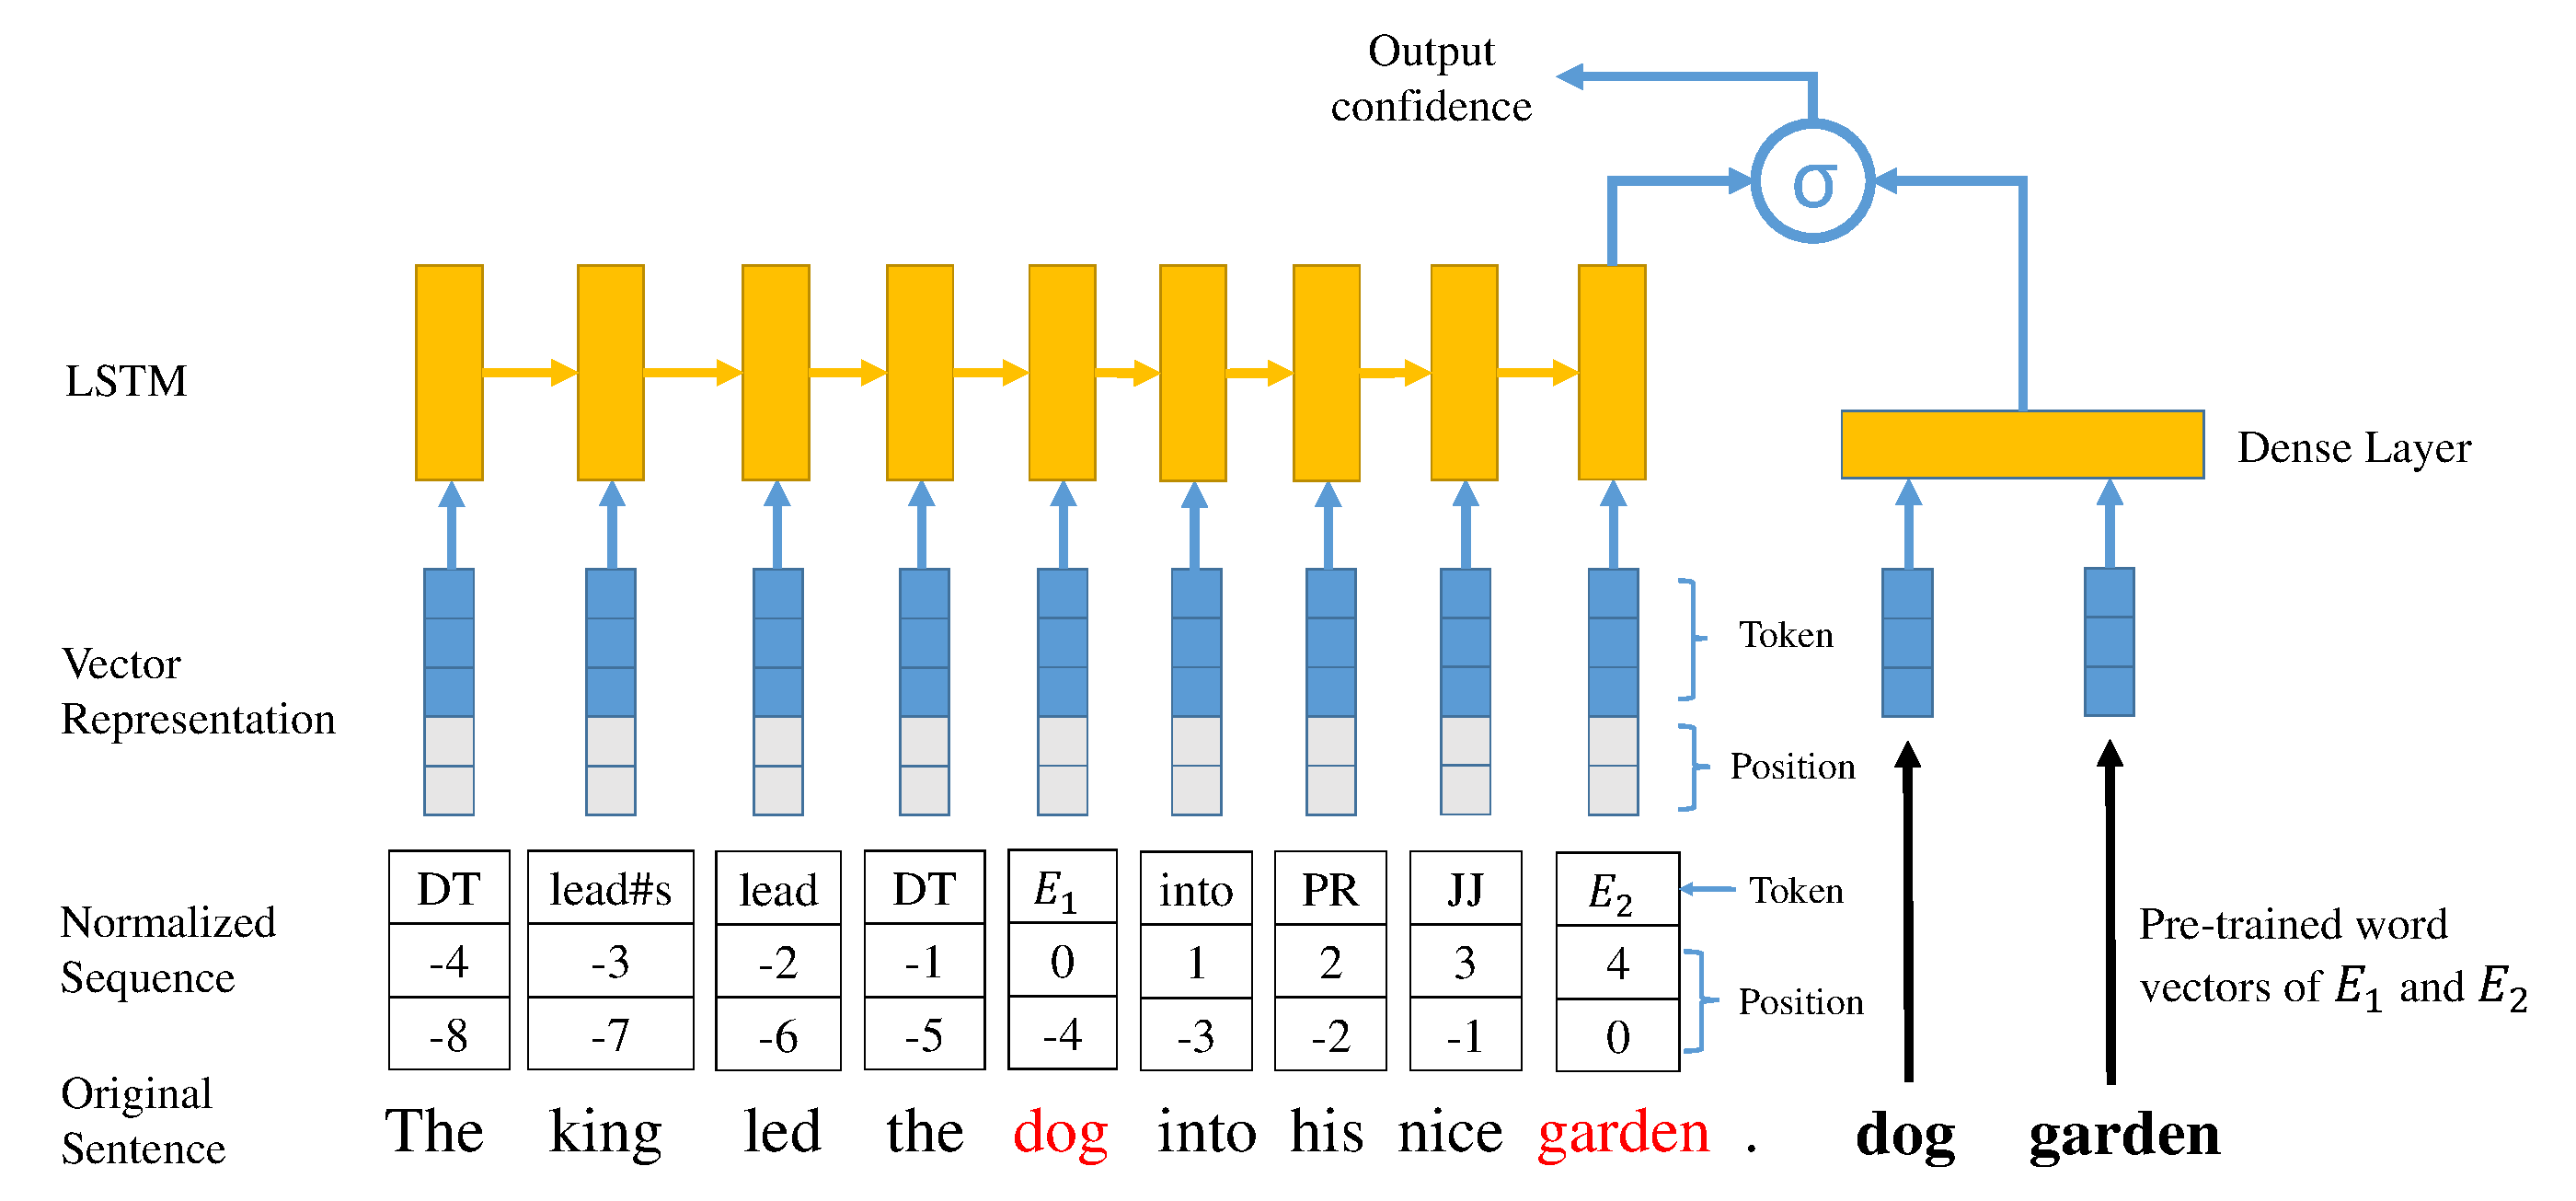
\epsfig{file=LSTM.pdf, width=0.9\textwidth}
	\caption{The proposed LSTM-based model}
	\label{fig:LSTM}
\end{figure*}

\subsubsection{Sentence Normalization}
%A LSTM layer is used to learn the representation of the sentence $s$.
%As for the form of input sentences, 
Using the original word sequence as of a sentence $s$ as input has two problems:
%(i) the original word sequence concerns little syntactical information;
(i) the irrelevant words in the sentence can take noise into model; 
(ii) the large vocabulary of original words induce too many parameters, which may cause over-fitting.
For example, given two sentences 
``\textit{The king led the dog into his nice garden.}'' and 
``\textit{A criminal led the dog into a poor garden.}''. 
The object pair is \textless \textit{dog, garden}\textgreater~in 
both sentences.
The two words ``\textit{lead}'' and ``\textit{into}'' are essential
for determining whether the object pair is located near, but they are not given more bias than other words. 
Also, the semantic differences between irrelevant words, such as ``king'' and ``criminal'', ``beautiful'' and ``poor'', are not useful to the co-location
relation between the ``dog'' and ``garden'', and 
thus tends to act as noise.

\begin{table}[th]
	\centering
	\small
	\begin{tabular}{l|l}
		\hline
		\textbf{Level}	&  \textbf{Examples}\\ 		\hline
		Objects	& $\textnormal{E}_1$, $\textnormal{E}_2$ \\ 		\hline
		Lemma & open, lead, into, ...\\ \hline 
		Dependency Role	& open\#s, open\#o, into\#o, ... \\ 		\hline 
		POS Tag	& DT, PR, CC, JJ, ... \\ 		\hline 
	\end{tabular}
	\caption{Examples of four types of tokens during sentence normalization. (\#s represents the subject of given verb or preposition, and \#o represents the object)}
	\label{tab:norm}
\end{table}

Considering above problems, we propose utilizing POS (Part-of-Speech) tags instead to capture more syntactical information and reduce the vocabulary size. 
However, solely doing this loses too much semantic dependency between the words. 
Thus, we propose a normalized sentence representation method merging the three most important and relevant kinds of information about each instance: lemma, POS tags and dependency role~\footnote{We utilize Stanford CoreNLP tool: \url{https://stanfordnlp.github.io/CoreNLP/}}. 

We first replace the two nouns in the object pair as $\textnormal{E}_1$ and $\textnormal{E}_2$, keep the lemmatized form of the original words for all the \textit{verbs, adverbs and prepositions}, which are highly relevant to describing physical scenes.
Then, we replace the \textit{subjects and direct objects} of the \textit{verbs and prepositions} (\texttt{nsubj, dobj} for verbs and \texttt{case} for prepositions in dependency parse tree) with special tokens indicating their dependency roles. 
For the remaining words, we simply use their POS tags to replace the originals. 
The four kinds of tokens are illustrated in ~\tabref{tab:norm}.
\tabref{tab:norm_eg} is a real example of our normalized sentence representation, where the object pair of interest is \textless \textit{dog, garden}\textgreater. 
\begin{table*}[!th]
	\small
	\centering
	\begin{tabular}{lllllllllllll}
		\hline
		\textit{The }&\textit{king }&\textit{opened }&\textit{the}&\textit{door}&\textit{and}& \textit{led}& \textit{the}& \textit{\textbf{dog} }& \textit{into }& \textit{his }& \textit{nice }& \textit{\textbf{garden}.}\\		 
		DT & open\#s & open & DT & open\#o & CC& lead& DT &$\textnormal{E}_1$ & into & PR & JJ& $\textnormal{E}_2$.\\	 \hline
	\end{tabular}
	\caption{Sentence Normalization Example}
	\label{tab:norm_eg}
\end{table*} 
\subsubsection{Model Training}
As shown in~\figref{fig:LSTM}, the bottom of the figure shows the original sentence, which is transformed to normalized sequence described above.
Apart from the normalized tokens of the original sequence, to capture more structural information, we also encode the distance from each token to $\textnormal E_1$ and $\textnormal E_2$.
{Such {word position embeddings} (position/distance features) are proposed by~\cite{zeng2014relation} with the intuition that information needed to determine the relation between two target nouns normally comes from words which are close to the target nouns.} 
%We adopt this feature because it can help LSTM keep track of the position of $\textnormal E_1$ and $\textnormal E_2$, better knowing \textit{where} the two object words are.
Then, we leverage LSTM to encode the whole sequence of the tokens of normalized representation plus position embedding. 
%\texttt{tanh} activation function is used following~\cite{xu2015classifying}. 

In the meantime, two pretrained GloVe word embeddings~\cite{pennington2014glove} of the original two physical object words are fed into a hidden dense layer. 
Finally, we concatenate both outputs and then use \texttt{sigmoid} activation function to obtain the final prediction.

{We choose to use the widely-used standard binary cross-entropy as our loss function, and
	RMSProp~\cite{hinton2012neural} is used as optimizer. Following~\cite{zaremba2014recurrent}, we add 0.5 dropout in LSTM as well as embedding layer, and utilize batch normalization~\cite{ioffe2015batch,cooijmans2016recurrent} for overfitting problem due to relatively small dataset.}

\section{\lnear\  Relation Extraction}
\label{sec:mine}
\figref{fig:overview} shows the overall workflow of our automatic framework to mine LocatedNear relations from raw text.
We first construct a vocabulary of physical objects and generate all candidate instances. 
For each sentence in the corpus, if a pair of physical objects $e_i$ and $e_j$ appear as nouns in a sentence $s$, then we apply our~\lnear\ relation classifier on this instance. 
The relation classifier yields a probabilistic score $s$
indicating the confidence of the existence of~\lnear~relation.
Finally, all scores of \textless $s$,$e_i$,$e_j$\textgreater~instances from the corpus are grouped by the object pairs and aggregated, where each object
pair is associated with a final score. 
Such mined physical pairs with scores can easily be integrated into existing commonsense knowledge base.

%\figref{fig:overview} shows the overall workflow of our framework for
%automatic extraction of \lnear\ relationship from text. 
More specifically, for each object pair \textless$e_i,e_j$\textgreater, 
we find all the $m$ sentences in our corpus mentioning both objects.
We classify the $m$ instances with the sentence-level relation classifier and get confidences for each instance, 
feed them into a function $f$ to obtain the final score 
of the object pair. 
%After scoring each pair, we can set a threshold to extract the new instances of \lnear\ relation.
There are five variants of the scoring functions:
\begin{align*}
	f_0=m \textnormal{,~~~~~}
	f_1=\sum_{k=1}^{m}\textnormal{conf}(s_k,e_i,e_j)&
	\textnormal{,~~}{~~~}f_2=\frac{1}{m}\sum_{k=1}^{m}\textnormal{conf}(s_k,e_i,e_j)
	\\
	f_3=\sum_{k=1}^{m}1_{\{\textnormal{conf}(s_k,e_i,e_j)>0.5\}}\textnormal{,~~~~~}&
	f_4=\frac{1}{m}\sum_{k=1}^{m}1_{ \{ \textnormal{conf}(s_k,e_i,e_j)>0.5 \}} \\
\end{align*}
\vspace{-20pt}
%$$f_0=m \\f_1=\sum_{k=1}^{m}\textnormal{conf}(s_k,e_i,e_j)\\ f_2=\frac{1}{m}\sum_{k=1}^{m}\textnormal{conf}(s_k,e_i,e_j)$, $f_3=\sum_{k=1}^{m}
%1_{\{\textnormal{conf}(s_k,e_i,e_j)>0.5\}}$$ and $	f_4=\frac{1}{m}\sum_{k=1}^{m} 
%1_{ \{ \textnormal{conf}(s_k,e_i,e_j)>0.5 \} }$.
\begin{figure*}[th]
	\centering
	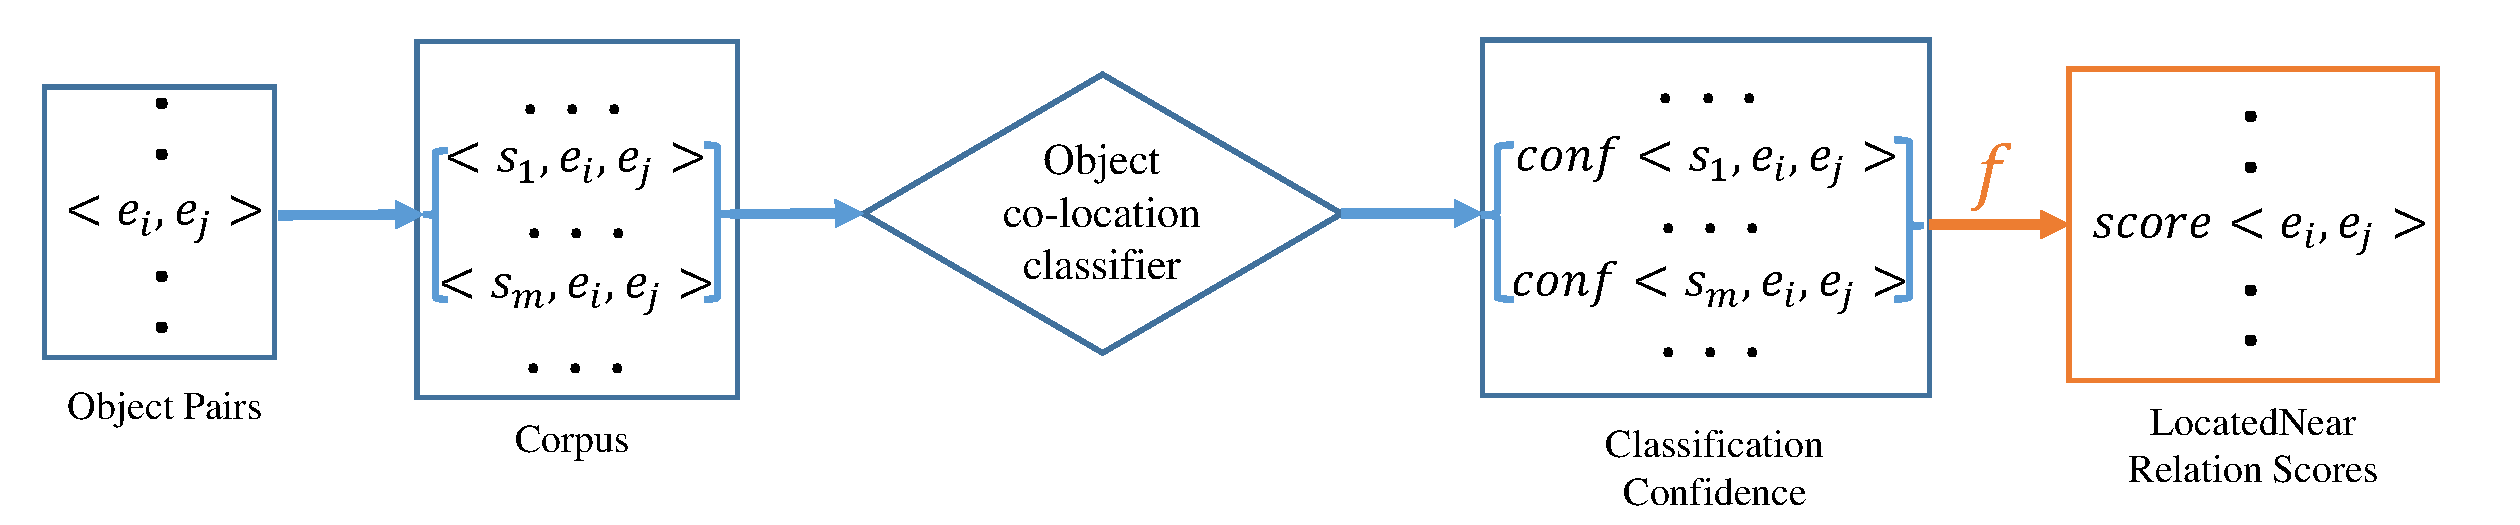
\epsfig{file=overflow.pdf, width=1\textwidth}
	\caption{Computing the \lnear\ scores of object pairs}
	\label{fig:overview}
\end{figure*}

%$f_1$ is the sum of the confidence of all the $m$ instances, $f_2$ is the average of the $m$ confidence scores, 
%$f_3$ is the number of the sentences whose confidence is higher than 0.5, 
%and $f_4$ is the ratio between the number of the sentences whose confidence is higher than 0.5 and $m$.

